\documentclass[
a4paper, % Paper size, use either a4paper or letterpaper
12pt, % Default font size, the template is designed to look good at 12pt so it's best not to change this
%unnumberedsections, % Uncomment for no section numbering
]{article}
\usepackage[a4paper,top=0.4cm, bottom=0.8cm, left=1.6cm, right=1.6cm]{geometry}

\usepackage{cmap} % make PDF files searchable and copy-able
\usepackage[utf8]{inputenc}
\usepackage[english,russian]{babel}

\usepackage{amssymb,amsmath}
\renewcommand {\phi}{\varphi}
\usepackage{mathtext}

\usepackage{libertine}
\usepackage[libertine]{newtxmath}

\usepackage{graphicx} % Required for inserting images
\graphicspath{{./img/}} % Destination of images
\usepackage{subcaption}

\usepackage{hyperref}

\usepackage{xcolor}



% opening
\title{
	\textcolor{cyan}{Отчет о выполнении лабораторной работы 1.4.5}
	\\
	Изучение колебаний струны
}
\author{Шубин Владислав, Байбулатов Амир}
%\date{Ноябрь 2023}

\begin{document}    
	
	\maketitle
	
	\section{Аннотация}
	
	В работе изучаются поперечные колебания стальной гитарной струны, натянутой горизонтально и закрепленной между двумя неподвижными зажимами; измеряются собственные частоты колебаний струны и проверяется условие образования стоячих волн; измеряется скорость распространения поперечных волн на струне и исследуется её зависимость от натяжения струны.
	
	Так как поперечные размеры струны малы по сравнению с длиной, то напряжение в струне может быть направлено только \textit{вдоль неё}. В \textit{натянутой струне} возникает \textit{поперечная упругость}, то есть способность сопротивляться всякому изменению формы, происходящему без изменения объёма. При вертикальном смещении произвольного элемента струны, возникают силы, действующие на соседние элементы, и в результате вся струна приходит в движение в вертикальной плоскости, т.е. возбуждение «бежит» по струне. Передача возбуждения представляет собой \textit{поперечные бегущие волны}, распространяющиеся с некоторой скоростью в обе стороны от места возбуждения. В ненатянутом состоянии струна не обладает свойством поперечной упругости, и поперечные волны на ней невозможны.
	
	\newpage
	
	\section{Теоретические сведения}
	
	\subsection{Уравнение волны на струне}
	Рассмотрим гибкую однородную струну, в которой создано натяжение \textit{T}, и получим дифференциальное уравнение, описывающее её малые поперечные свободные колебания. Отметим, что, если струна расположена горизонтально в поле тяжести, величина \textit{T} должна быть достаточна для того, чтобы в состоянии равновесия струна \textit{не провисала}, т.е. сила натяжения должна существенно превышать вес струны.
	
	Направим ось $x$ вдоль струны в положении равновесия. Форму струны будем описывать функцией $y(x,t)$, определяющей её вертикальное смещение струны в точке $x$ в момент времени $t$ (см. рис. \ref{graph}).
	\begin{figure}[h]
		\centering{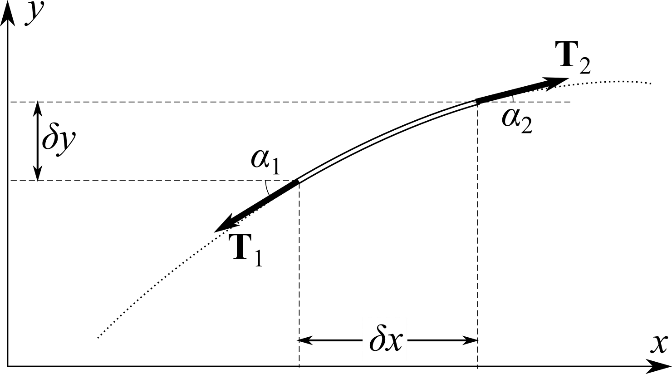
\includegraphics[scale=0.6]{oscillation_graph.png}}
		\caption{К выводу уравнения колебаний струны}
		\label{graph}
	\end{figure}
	
	Рассмотрим элементарный участок струны, находящийся в точке $x$, имеющий длину $\delta x$ и массу
	\begin{equation}
		\delta m = \rho_l \delta x, \; \text{где $\rho_l$ [кг/м] - \textit{погонная плотность струны}}
	\end{equation}
	При отклонении от равновесия на выделенный элемент действуют силы натяжения $T_1$ и $T_2$, направленные по касательной к струне.
	
	Тогда по II закону Ньютона в проекциях на ось $y$ для элемента получим:
	\begin{equation}
		\delta m \frac{\partial^2 y}{\partial t^2}= -T_1 \sin{\alpha_1} + T_2\sin{\alpha_2}
	\end{equation}
	Так как амплитуда колебаний невелика, то можно пренебречь добавочным напряжением, возникающим из-за \textit{удлинения} элементов струны и считать силу $T$ натяжения нити постоянной по модулю. Также можно считать углы отклонения $\alpha$ струны от оси $x$ малыми, поэтому $\tg{\alpha} \approx \sin{\alpha} \approx \alpha$.
	
	Устремим $\delta x$ к нулю и найдем окончательно \textit{уравнение свободных малых поперечных колебаний струны:}
	\begin{equation}
		\rho_l \frac{\partial^2 y}{\partial{t^2}} \approx T\frac{\partial{\alpha}}{x} = u^2\frac{\partial^2 y}{\partial{t^2}}, \quad \left(u = \sqrt{\frac{T}{\rho}}\right)
	\end{equation}
	
	\begin{equation}\label{wave}
			\frac{\partial^2 y}{\partial t^2} = u^2 \frac{\partial^2 y}{\partial x^2} \quad - \quad \text{волновое уравнение.}
	\end{equation}
	
	\newpage
	
	\subsection{Бегущие волны}
	Рассмотрим \textit{произвольную} функцию вида $y = f(x - ut)$. Подставляя её в уравнение \eqref{wave}, убеждаемся, что она является решением при любом $f$:
	\begin{equation}
		\frac{\partial^2 f}{\partial t^2} = (-u)^2 f'' = u^2 \frac{\partial^2 f}{\partial x^2}, \; \text{где штрих обозначает производную по аргументу $\xi = x - ut$ .}
	\end{equation}
	Считая аргумент функции $f$ постоянным $x - ut = const$ и дифференцируя по времени получим: $dx = udt = 0$, откуда $\frac{dx}{dt} = u$.
	
	Общее же решение волнового уравнения представимо в виде суперпозиции двух волн произвольной формы, бегущих вдоль оси $x$ со скоростями $\pm u$:
	\begin{equation}
		y(x,t) = y_1(x-ut) + y_2(x+ut), \quad где u - \text{скорость волны, $y_1$ и $y_2$ - произвольные функции}
	\end{equation}
	Вид $y_1$ и $y_2$ в конкретной задаче определяется из начальных и граничных условий.
	
	В данной работе будут изучаться \textit{гармонические волны}:
	\begin{equation}\label{harmonic}
		y(x,t) = a \cos\left[k(x - ut)\right] + b \cos\left[k(x+ut)\right] = a\cos\left(\omega t - kx\right) + b\cos\left(\omega t + kx\right)
	\end{equation}
	Здесь $\omega$ - циклическая частота колебаний, а $k = \frac{\omega}{u} = \frac{2\pi}{\lambda}$ - \textit{пространственная частота} волны. ($\lambda$ - длина волны).
	
	\newpage
	
	\subsection{Собственные колебания струны. Стоячие волны}
	
	Найдем вид свободных колебаний струны с \textit{закрепленными концами}. Пусть струна закреплена в точках $x = 0$ и $x = L$. Тогда из условия $y(0, t) = 0 \ (\forall t)$, и уравнения \ref{harmonic} получим:
	\begin{equation}
		a \cos(\omega t) + b \cos(\omega t) = 0 \Rightarrow a = -b
	\end{equation} 
	Тогда:
	\begin{equation}\label{harmonic_shortened}
		y(x,t) = a(\cos(\omega t - k x) - \cos(\omega t + k x)) = 2 a \sin{kx} \cdot \sin{\omega t}
	\end{equation}
	
	Видно, что данная волна получается в результате суперпозиции двух гармонических бегущих навстречу друг другу волн с равными амплитудами. Такая волна называется \textit{стоячей}. Вся струна колеблется с циклической частотой $\omega$. При этом амплитуда колебаний распределена по струне по закону: $y_m(x) = 2 a \sin{kx}$. В точках, где $\sin{kx} = 1$, амплитуда колебаний максимальна (\textit{пучности волны}). Точки, у которых $\sin{kx} = 0$ не колеблются вовсе (\textit{узлы волны}). Точки струны между двумя соседними узлами всегда колеблются в одной фазе, то есть в любой момент времени их скорости сонаправлены.
		
	Используем второе граничное условие $y(L, t) = 0 \ (\forall t)$ (точки крепления
	струны должны быть узлами стоячей волны):
	\begin{equation}
		\sin{kL} = 0 \Rightarrow kL = n\frac{\pi}{2}, \quad n \in \mathbb {N} 
	\end{equation}
	Тогда:
	\begin{equation}
		\lambda_n = \frac{2L}{n}, \quad n \in \mathbb{N}
	\end{equation}
	Как видно, параметр $n$ определяет число полуволн (то есть пучностей), которые умещаются на струне. Так как длина волны однозначно связана с её частотой, то струна может колебаться только с определёнными частотами:
	\begin{equation}\label{eq12}
		\nu_n = \frac{u}{2L} n
	\end{equation}
	
	\begin{figure}[h]
		\centering{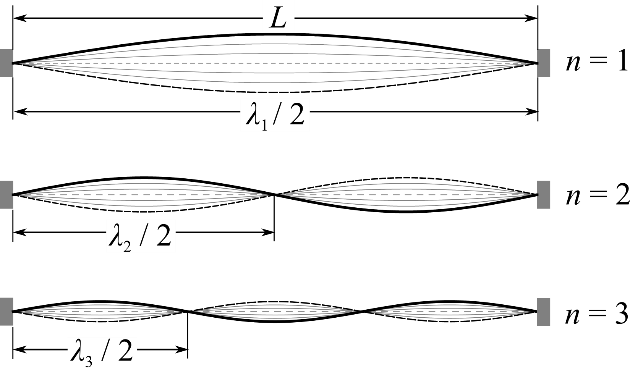
\includegraphics[scale=0.6]{standing_waves.png}}
		\caption{Стоячие волны (собственные моды колебаний струны) для n = 1, 2, 3}
		\label{standing_waves}
	\end{figure}
	
	Спектр собственных частот $\nu_n$ колебаний струны зависит только от её натяжения, линейной плотности и длины и, в случае малых гармонических колебаний, не зависит от модуля Юнга материала струны.
	
	\newpage
	
	\subsection{Возбуждение колебаний струны. Резонанс}
	
	При колебаниях реальной струны всегда имеет место потеря энергии. Поддержание незатухающих
	колебаний в струне может осуществляться точечным источником, в качестве которого в данной работе используется электромагнитный вибратор. 
	Для эффективной раскачки колебаний используется явление резонанса - необходимо, чтобы вынуждающая частота $\nu$ вибратора совпала с одной из собственных частот $\nu_n$ струны. Тогда в любой момент времени потери энергии будут компенсироваться поступающей от воздбудителя колебаний энергией, процесс становится стационарным и можно наблюдать стоячие волны.
	
	Также стоит отметить, что в идеальном случае поток энергии вдоль стоячей волны отсутствует (в каждом участке между узлами кинетическая энергия переходит в потенциальную и наоборот). Однако, энергия от вибратора должна каким-то образом доходить до удалённых от него частей струны, поэтому в реальности помимо стоячей волны, есть ещё и малая бегущая компонента, которая и переносит энергию источника. Если потери энергии за период малы по сравнению с запасом колебательной энергии в струне, то искажение стоячих волн бегущей волной не существенно — наложение бегущей волны малой амплитуды на стоячую визуально приводит к незначительному «размытию» узлов (амплитуда колебаний в узлах совпадает с амплитудой бегущей компоненты волны).
	
	Для достижения максимальной раскачки колебаний, необходимо располагать возбуждающий контакт вблизи узловый точки (но не строго в ней). Действительно, предположим, что вибратор способен раскачать соответствующий элемент струны до амплитуды $A$. Если $x_0$ - расстояние от него до пучности, то из формулы \eqref{harmonic_shortened}:
	\[A = 2a \sin{kx_0} \Rightarrow a = \frac{A}{2\sin{kx_0}} \]
	Отсюда видно, что расстояние $x_0$ следует устремлять к нулю.
	
	Наконец отметим, что в ходе работы необходимо добиться того, чтобы колебания были \textit{линейно поляризованы}, то есть чтобы струна колебалась в одной плоскости. Также необходимо обеспечить малость амплитуды колебаний - в противном случае волновое уравнение \eqref{wave} будет неприменимо.
		
	\newpage
	
	\section{Оборудование и инструментальные погрешности}
	\textbf{Оборудование}: звуковой генератор, двухканальный осциллограф, частотомер, набор грузов, станина, с закрепленной на ней струной.

	\begin{itemize}
		\item Точность измерения массы грузов $\pm 0,1$ г.
		\item Точность измерения с помощью линейки $\pm 0,1$ cм.
		\item Точность измерения частот $\pm 0,1$ Гц.
	\end{itemize}
	
	%\newpage
	
	\section{Результаты измерений и обработка данных}
	
	\subsection{Описание экспериментальной установки}
	Схема установки приведена на \ref{experimantal}. Стальная гитарная струна 1 закрепляется в горизонтальном положении между двумя стойками с зажимами 2 и 3, расположенными на массивной станине 4. Один конец струны
	закреплен в зажиме 2 неподвижно. К противоположному концу струны, перекинутому через блок, прикреплена платформа с грузами 5, создающими натяжение струны. Зажим 3 можно передвигать по станине, устанавливая требуемую длину струны. Возбуждение и регистрация колебаний струны осуществляются с помощью электромагнитных датчиков (вибраторов), расположенных на станине под струной. Электромагнитный датчик 6 подключен к звуковому генератору 7 и служит для возбуждения колебаний 10 струны, частота которых измеряется с помощью частотомера 10 (в некоторых установках частотомер встроен в генератор). Колебания струны регистрируются с помощью электромагнитного датчика 8, сигнал с которого передается на вход осциллографа 9. Разъёмы, через которые датчики с помощью кабелей соединяются с генератором и осциллографом, расположены на корпусе станины.
	
	\begin{figure}[h]
		\centering{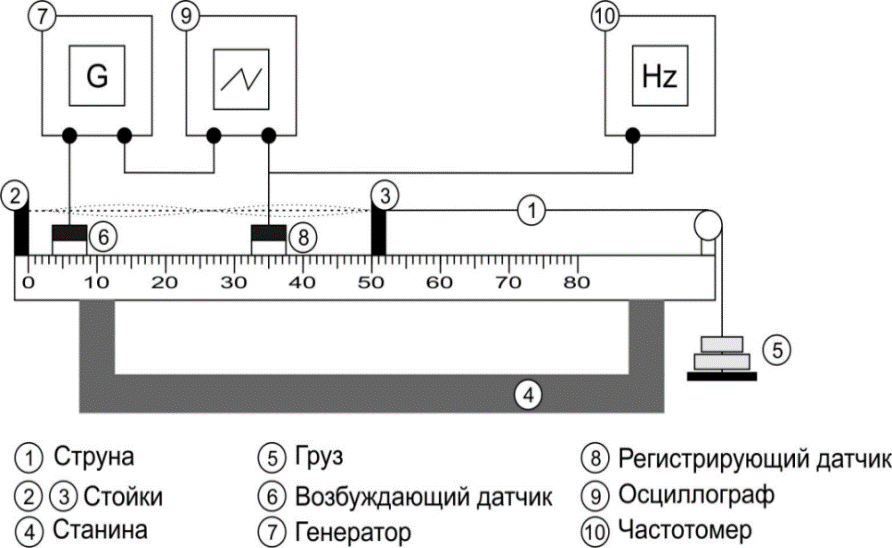
\includegraphics[scale=0.4]{experimental.png}}
		\caption{Экспериментальная установка}
		\label{experimantal}
	\end{figure}
	
	%\newpage
	
	\subsection{Характеристики системы:}
	
	$L = 0.5\pm 0,001$ м,\\
	$\rho = 568,4 * 10^{-6}$ г/м
	
	\subsection{Предварительные расчеты:}
	
	$u = \sqrt{\frac{T}{\rho}} \approx 120 \: \text{м/c}$\\
	$\nu_1 \approx 120 \: \text{Гц}$
	
	\newpage
	
	\subsection{Наблюдения:}
	
	\begin{table}[h]
		\centering
		\begin{tabular}{|c|c|c|c|}
			\hline
			n & 1 & 2 & 3  \\
			\hline
			$\nu_n, Гц$ & 128 & 261 & 391 \\
			\hline
		\end{tabular}
		\caption{Результаты определения частот 3-х гармоник по частотометру}
	\end{table}
	
	\subsection{Измерения:}
	
	\begin{table}[h]
		\centering
		\begin{tabular}{|c|c|c|c|}
			\hline
			n & 1 & 2 & 3  \\
			\hline
			$M_n$, г & 835.4 & 1322.8 & 1820 \\
			\hline
		\end{tabular}
		\caption{Массы нагрузки}
	\end{table}
	
	
	\begin{table}[h]
		\centering
		\begin{tabular}{|c|c|c|c|c|c|c|}
			\hline
			N изм. & 1 & 2 & 3 & 4 & 5 & 6 \\
			\hline
			$\nu$, Гц & 130.0 & 259.0 & 388.0 & 519.0 & 650.0 & 780.0 \\
			\hline
		\end{tabular}
		\caption{Результаты измерений частот 6-ти гармоник для $M_1$}
	\end{table}
	
	\begin{table}[h!]
		\centering
		\begin{tabular}{|c|c|c|c|c|c|c|}
			\hline
			N изм. & 1 & 2 & 3 & 4 & 5 & 6 \\
			\hline
			$\nu$, Гц & 159.0 & 319.0 & 478.0 & 638.0 & 799.0 & 960.0 \\
			\hline
		\end{tabular}
		\caption{Результаты измерений частот 6-ти гармоник для $M_2$}
	\end{table}
	
	\begin{table}[h!]
		\centering
		\begin{tabular}{|c|c|c|c|c|c|c|}
			\hline
			N изм. & 1 & 2 & 3 & 4 & 5 & 6 \\
			\hline
			$\nu$, Гц & 185.0 & 371.0 & 556.0 & 742.0 & 928.0 & 1116.0 \\
			\hline
		\end{tabular}
		\caption{Результаты измерений частот 6-ти гармоник для $M_3$}
	\end{table}
	
	
	Построим графики зависимостей $\nu_n(n)$ для каждого из трёх опытов и аппроксимируем их линейной функцией по МНК. Результаты - на \ref{mnk_graph}.
	
	\begin{figure}[h!]
		\centering{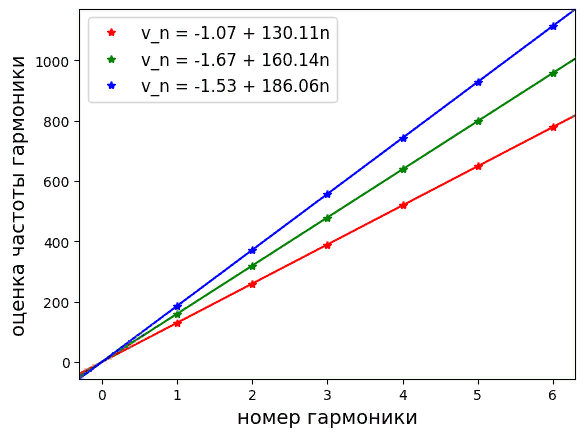
\includegraphics[scale=0.68]{graph_mnk.png}}
		\caption{Графики зависимостей $\nu_n(n)$ и их аппроксимация линейной функцией по МНК}
		\label{mnk_graph}
	\end{figure}
	
	\newpage
	
	Зная угловые коэффициенты $k$ этих зависимостей, определим скорость распространения волн в струне в каждом случае, как:
	\[u = 2kL \]
	
	\begin{equation}
		k=\frac{\langle n\nu\rangle-\langle n\rangle \langle \nu\rangle}{\langle n^2\rangle - \langle n\rangle^2},
	\end{equation}
	
	\begin{equation}
		\sigma_k^\text{случ}=\frac{1}{\sqrt{N}}\sqrt{\frac{\langle \nu^2 \rangle - \langle \nu \rangle^2}{\langle n^2 \rangle - \langle n \rangle^2} - k^2  },
	\end{equation}
	
	\begin{equation}
		\sigma_k^{\text{сист}} = \sqrt{ \varepsilon_\nu^2 + \varepsilon_l^2 }
	\end{equation}
	
	\begin{equation}
		\sigma_k = \sqrt{\sigma_\text{случ}^2 + \sigma_\text{сист}^2}
	\end{equation}
	
	Посчитав все погрешности, коэффиценты наклона и из них найдем $u$, получаем таблицу:
	
	\begin{table}[h]
		\begin{center}
			\begin{tabular}{|c|c|c|c|}
				\hline
				$T\text{, Н}$ & 8.2 & 13.0 & 17.8\\ \hline
				$u\text{, м/с}$  & 130,1 & 160,1 & 186,1 \\ \hline
				$\sigma_{u}^{\text{случ}} \text{, м/с}$ & 0.42 & 0.37 & 0.43  \\ \hline
				$\sigma_{u}^{\text{сист}} \text{, м/с}$ & 2.1 & 2.1 & 1.9 \\ \hline
				$\sigma_{u} \text{, м/с}$ & 2.2 & 2.1 & 1.9 \\ \hline
			\end{tabular}
			\caption{Полученные скорости с погрешностями}
		\end{center}
	\end{table}
	
	\noindent
	Средняя относительная погрешность измерения скорости распространения колебаний $\varepsilon_u \approx 1,3\% $. Полученные значения скорости:
	
	\begin{itemize}
		\item $T = 8,2$ Н  $\quad u = (130,1 \pm 2,2)$, м/с
		\item  $T = 13,0$ Н  $\quad u = (160,1 \pm 2,1)$, м/с
		\item  $T = 17,8$ Н  $\quad u = (186,1 \pm 1,9)$, м/с
	\end{itemize}
	
	С помощью полученных данных построим график зависимости $u^2(T)$, для того, чтобы найти погонную плотность струны $ \rho_l $.
	
	\begin{figure}[h!]
		\begin{center}
			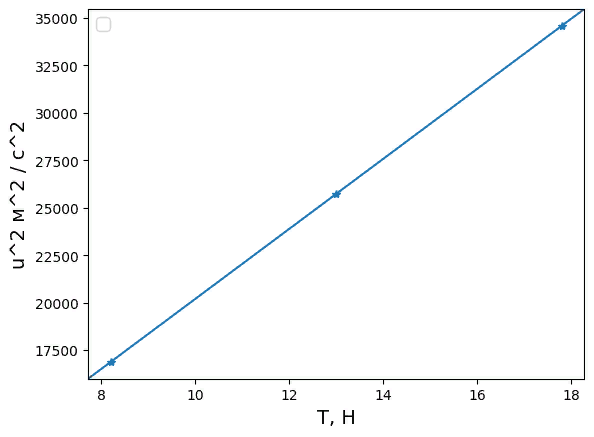
\includegraphics[scale=0.96]{graph_u_T.png}
			\caption{Зависимость $ u^2 $ от $ T $}
			\label{graph_u_T}
		\end{center}
	\end{figure}
	
	С помощью формулы скорости через натяжение и погонную плотность, можно понять, что коэффицент наклона $k$, для графика \ref{graph_u_T}, будет равен: $k = \dfrac{1}{\rho_l}$.
	
	График был построен по МНК, а значит $k$ и его погрешность можно найти по формулам:
	
	\begin{equation}
		k=\frac{\langle Tu^2\rangle-\langle T\rangle \langle u^2\rangle}{\langle T^2\rangle - \langle T\rangle^2} \approx 1811.5 \text{, $\dfrac{\text{м}}{\text{кг}}$},
	\end{equation}
	
	\begin{equation}
		\sigma_k^\text{случ}=\frac{1}{\sqrt{N}}\sqrt{\frac{\langle u^4 \rangle - \langle u^2 \rangle^2}{\langle T^2 \rangle - \langle T \rangle^2} - k^2  } \approx 17.8 \text{, $\dfrac{\text{м}}{\text{кг}}$},
	\end{equation}
	
	\begin{equation}
		\sigma_k^{\text{сист}} = \sqrt{ \varepsilon_{u^2}^2 + \varepsilon_T^2 } \approx 40,2\text{, $\dfrac{\text{м}}{\text{кг}}$},
	\end{equation}
	
	\begin{equation}
		\sigma_k = \sqrt{\sigma_\text{случ}^2 + \sigma_\text{сист}^2} \approx 44,0 \text{, $\dfrac{\text{м}}{\text{кг}}$},
	\end{equation}
	
	Таким образом $k = 1811.5 \pm 44,0 \left({ \dfrac{\text{м}}{\text{кг}}}\right) $.
	Тогда $\rho_l = 552.0 \pm 13.5 \left({ \dfrac{\text{мг}}{\text{м}}}\right)$.
	
	Полученное значение близко к истинному значению погонной плостности струны, которая равняется $\rho^{\text{ист}}_l = 568,4\left({ \dfrac{\text{мг}}{\text{м}}}\right) $. 
	
	\newpage
	
	\section{Заключение}
	\begin{enumerate}
		\item
		Во время выполнения работы было подтверждено несколько теоретических зависимостей между физическими величинами. С точностью $\varepsilon_{\nu_{1}} = 0,015$ подтверждена формула для определения частот гармоники струны. С точностью  $\varepsilon_{u} = 0,013$ подтверждена формула для определения скорости распространения волны в твердом теле под действием внешней силы.
		\item
		Полученные графики имеют вид, предсказанный теоретически.
		\item
		Отличие значения линейной плотности струны от указанного на установке более чем на погрешность, может быть связано с неточностью определения собственных частот $\nu_n$ из-за возникновения нелинейных эффектов при резонансе, и, как следствие, неточностью в определении скорости распространения $u$ волны в струне.
	\end{enumerate}
	
	
\end{document}
